\documentclass[12pt]{article}
\usepackage[margin=1.0in]{geometry}
\usepackage{graphicx}
\usepackage{subcaption}
\usepackage{cleveref}
\usepackage{indentfirst}
\usepackage{amsmath}
\usepackage{listings}
\usepackage[title]{appendix}
\usepackage{siunitx} % Required for alignment
\usepackage{mdframed}

\begin{document}

	
\begin{center}
	\huge{Exploring the Effects of the Adaptive Cosine Estimator on Convolutional Neural Network Performance for Hyperspectral Imagery Classification} \\
	\vspace{5mm}
	\large{Alex Hurt}
\end{center}

%1) ABSTRACT. why care, what method did you use, what data did you explore, what did you find!
%
\section{Abstract}

Hyperspectral Imagery (HSI) Classification is a difficult but important task in Remote Sensing.
%
As hyperspectral sensors become more popular, the ability to perform classification at the hyperspectral level will grow more and more important.
%
HSI has many challenges that other image sources (i.e. RGB) do not have, such as labeling at the pixel level rather than image level and a so-called curse of dimensionality.
%
In recent years, several researchers have attempted to perform HSI classification with a variety of methods.
%
With the rise of deep learning, one of the most popular methods for HSI classification is Convolutional Neural Networks (CNN).
%
While HSI have several inherent challenges, so too do Convolutional Neural Networks, and understanding the limitations of CNN is critical to building a well performing classifier.
%
Recently, researchers have tried several tweaks to the standard CNN to improve HSI classification performance, such as using deformable convolutions by Zhu \textit{et al.} \cite{zhu_deformable_2018}. 
%
Another approach was taken by Paoletti \textit{et al.}, who used a CNN combined with capsule networks for HSI classification \cite{paoletti_capsule_2018}.

While numerous approaches have been taken for HSI classification, most techniques do not utilize the amount of spectral information contained in HSI when performing classification.
%
To that end, I will utilize a method of detection in HSI given sample object signatures, known as the Adaptive Cosine Estimator (ACE).
%
ACE allows detection and produces scoring at the pixel level within HSI given the signature of the objects of interest. 
%
In this project, I will combine the ACE technique with a CNN to produce a custom neural network architecture that involves preprocessing samples with ACE, named \textit{ACENet}.
%
ACENet combines the spectral classification methods of ACE with the spatial classification methods utilized by CNN to produce an architecture that can better classify HSI.
%
More details of this new architecture are described in Section \ref{sec:methods}.
%
Following the description of methods, I describe the data used for experimentation in Section \ref{sec:data} and then the design, results, and analysis of experiments in \ref{sec:experiments} before drawing final conclusions in Section \ref{sec:conclusion}.


%2) METHODS. describe your algorithm(s). your goal, show me you KNOW it
%
\section{Methods}\label{sec:methods}
To explore the effects of ACE on CNN Performance, I first move to introduce the data preprocessing that is performed prior to input to the CNN.
%
Since most hyperspectral datasets are labeled at the pixel label, the first step of preprocessing is to extract patches from the dataset.
%
To do this, parameters of window size and stride are selected and then used to extract patches of size window size by window size, and then sliding a number of pixels defined by stride.
%
Each patch is then normalized between 0 and 1 and fed into ACENet.

The ACENet architecture has two different modes: with or without ACE.
%
The only difference between the two is in the non-ACE mode, each patch is fed in raw and the input size to the first convolutional layer is $(w \times w \times b)$ where $w$ is the window size and $b$ is the number of bands in the hyperspectral dataset.
%
Meanwhile, the ACE mode has another step between preprocessing and the first convoutional layer known as the ACELayer.
%
The ACELayer uses the dataset and ground truth to calculate a mean signal for each class in the dataset.
%
ACE is then run on each patch with each class's mean signal as the target signal. 
%
The ACE algorithm is based upon the ACE equation:
$$
\text{ace}(x;(\mu,\Sigma)) = \frac{ \left[s^T \Sigma^{-1} x\right]^2 }{\left[s^T \Sigma^{-1} s\right] \left[x^T \Sigma^{-1} x\right]}
$$
%
There are two forms of ACE: one that calculates $\mu$ and $\Sigma$ for the entire input signal, and one that calculates them for a window and then slides across the input signal.
%
For this project, the second form of ACE, known as ACE Local, is used, and the ACE window size is fixed at 3 due to the small input signals being only between 5x5 and 11x11.
%
The resulting matrices are concatenated to form a single input sample with shape $(w \times w \times n)$ where $w$ is the window size and $n$ is the number of classes, which is also the input shape of the first convolutional layer.
%
Both modes of ACENet have the same number of samples, but the ACE enabled mode has a reduction of dimensionality due to the number of classes being less than number of bands in HSI, but also has added computation of transforming samples from HSI pixels to the concatenation of ACE results.

Both ACE enabled and ACE disabled modes of ACENet have identical architectures beginning at the first convolutional layer.
%
The framework developed for this architecture is parameterized to allow for an arbitrary number of convolutional layers so that an optimal setting may be found for a given dataset.
%
Following the final convolutional layer, there is a single Max Pooling layer that feeds into a flattening layer.
%
Now that all feature extraction is finished, the flattened features are fed into the first fully connected layer composed of 256 units.
%
Next, a 25\% dropout layer is added in an attempt to add generalizability and improve cross validation performance.
%
Another fully connected layer follows the dropout layer before the final softmax layer for classification.



%3) DATA. document your data
%
\section{Data}\label{sec:data}
For this project, I chose to use the ever popular HSI benchmark dataset Indian Pines (IP) \cite{IP}.
%
IP is a HSI dataset composed of 220 hyperspectral bands that was collected in 1992 and has been used in a variety of research.
%
The dataset has shape of 144x144, and is one of few HSI datasets that has excellent pixel level ground truth data.
%
Use of this dataset will allow for easy comparison of this method with other methods due to the high popularity of IP.
%
The IP dataset is distributed as MatLab files and has 16 agricultural classes within it.

%4) EXPERIMENTS and RESULTS. what did you run and what did you find. Yes, document, but I want to see your ANALYSIS!
%
\section{Experiments}\label{sec:experiments}

In an effort to test the usability of ACENet, several experiments were run with several different parameters, both in ACE enabled and ACE disabled modes. 
%
The first set of experiments were done to test how stride and window size affected validation testing of CNN on HSI in general, and then another was run to explore how those same two parameters affected results with ACE enabled.
%
After finding ideal sets of window and stride sizes and exploring how ACE enabled CNN perform against Non-ACE enabled CNN, I investigate what the optimal number of convolutional layers is for feature extraction in HSI imagery.
%
All experiments are run using the IP dataset and are run using a Keras/TensorFlow software stack on a server with 4 NVIDIA Tesla V100s and 80 logical processors.
%
Network parameters were held constant with an initial learning rate of 0.01 and decay of 1e-6 along with a momentum of 0.9 in a Stochastic Gradient Descent (SGD) optimizer and categorical cross entropy loss function.
% 

\subsection{Varied Window and Stride Sizes}
Due to the pixel level labeling seen in the IP dataset and the necessity of CNN to have some NxN patch of input, it is a useful task to vary the input patch size and observe how that change impacts CNN performance. 
%
A balance must be struck between computational complexity and context around a pixel.
%
If the window size is too small, then there is not enough context, and performance is hindered, while a window size too large will result in more complex calculations with higher training times and may lead to a performance hit as well depending if the chosen size contains too much context relative to the labeled pixel.
%
To that end, I adjust the window size $w$ from 5x5 up to 11x11 in 2x2 increments, and set the stride for each experiment to $\lfloor\frac{w}{2}\rfloor$. 
%
I set ACENet to run in ACE disabled mode, and use 15 convolutional layers and train for 100 epochs on 80\% of the data.
%
I use the remaining 20\% of validation data, and the results of this experiment are shown in Figure \ref{figure:noace}.

\begin{figure*}[t]

	\centering
	\caption{ACENet results on IP after 80/20 validation split using various window sizes}
	\label{figure:noace}
	\begin{subfigure}{0.45\linewidth}
		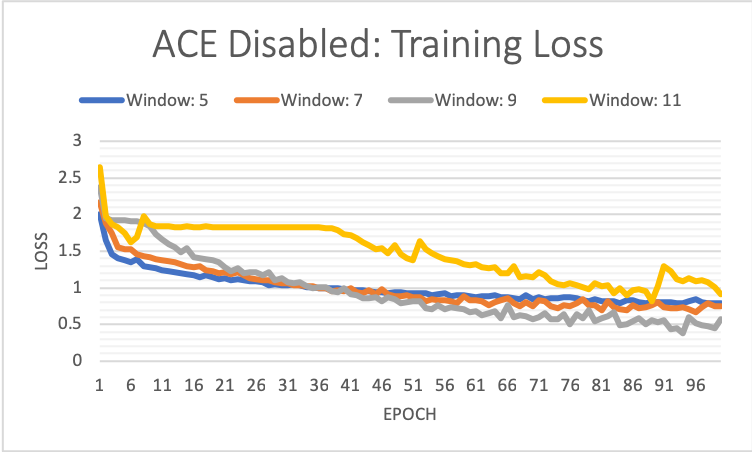
\includegraphics[width=\linewidth]{ace-disabled-loss.png}
		\caption{ACE Disabled Training Loss}
	\end{subfigure}
	\hfill
	\begin{subfigure}{0.45\linewidth}
		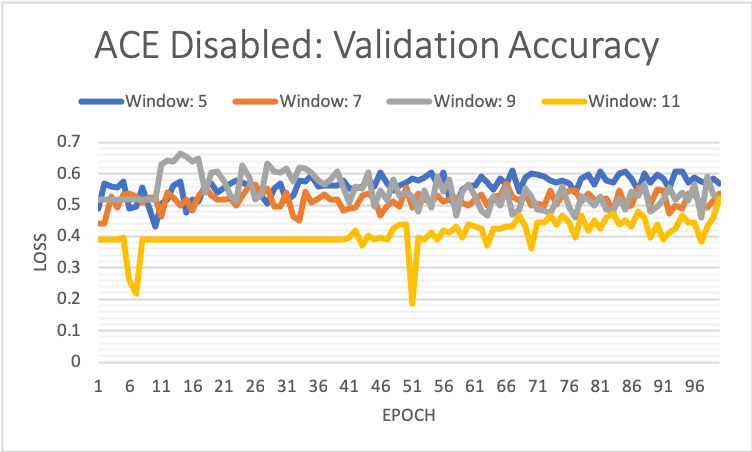
\includegraphics[width=\linewidth]{ace-disabled-valacc.png}
		\caption{ACE Disabled Validation Accuracy}		
	\end{subfigure}


	\begin{subfigure}{0.45\linewidth}
		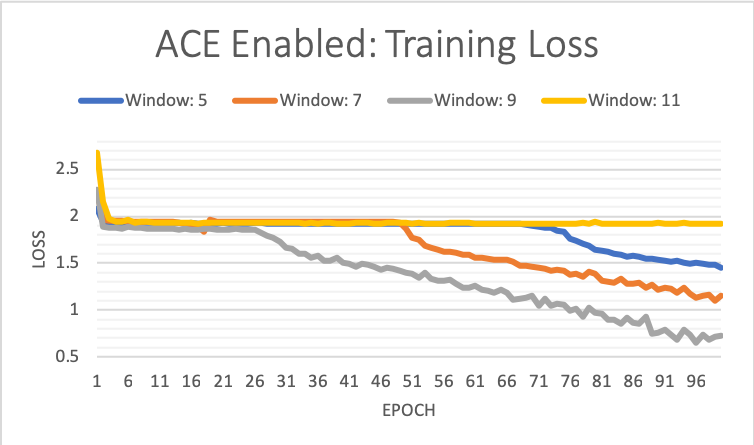
\includegraphics[width=\linewidth]{ace-enabled-loss.png}
		\caption{ACE Enabled Training Loss}
	\end{subfigure}
	\hfill
	\begin{subfigure}{0.45\linewidth}
		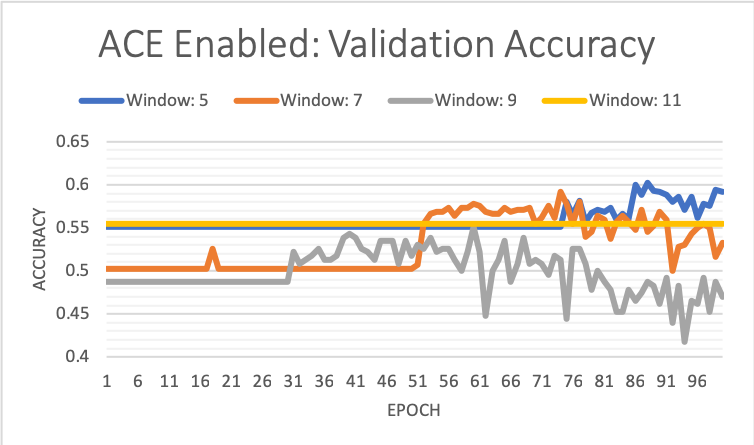
\includegraphics[width=\linewidth]{ace-enabled-valacc.png}
		\caption{ACE Enabled Validation Accuracy}		
	\end{subfigure}
\end{figure*}


The results of ACE Disabled HSI classification are not extraordinary.
%
The best validation accuracy is a measly 0.664, which occurs with a window size of 9 after 14 epochs of training.
%
The loss in ACE disabled classification is highly irregular, with loss spiking at various epochs.
%
The expected behavior of loss would be a smooth downward sloping curve, but instead we see several increases in loss between epochs of training.
%
The training loss' behavior is mirrored in the validation accuracy. 
%
I was hoping, even expecting, to see the validation accuracy slowly increase over epochs of training. 
%
However, the validation accuracy is jumpy and oscillating, without any standard behavior, which indicates a lack of network convergence.
%
This could perhaps be rectified with more training (more epochs) or a change of hyper-parameters.

While the results show a lack fo convergence, they still show that the window size is an important factor in validation accuracy for CNN classification of HSI.
%
The loss drop seen for window size of 9 is the closest to regular of the four window sizes, and the highest loss throughout training was for window size 11.
%
The lack of drop in loss shows that the CNN is not learning the data in 100 epochs as the smaller window sizes, and this translates to the lowest validation accuracy for all 100 epochs.
%
Unfortunately, the direct relationship between training loss and validation accuracy breaks with window size of 5.
%
The best performing window size was 5, but the best window size in terms of training loss was 9. 
%
This result is confusing because with a window size of 5, the ratio of context to data is 25:1, but for window size of 9, that ratio is 81:1, more than 3x larger.

After reviewing the results of ACE Enabled CNN classification, we see that the network is greatly impacted by window size.
%
We see a nearly fixed training loss and validation accuracy for the Window Size 11 experiment. 
%
This indicates that 11 is too high and has too much context.
%
The results also show that in regards to training loss, a window size of 9 is optimal, but for validation accuracy, the optimal window size is 5.
%
Overall, since for both ACE enabled and ACE disabled CNN, the best window size turned out to be 5, indicating that less context is better for CNN classification performance.


\subsection{ACE Enabled vs. ACE Disabled}


\begin{figure*}[t]
	
	\centering
	\caption{ACENet results on IP after 80/20 validation split with and without ACE Enabled}
	\label{figure:acevnoace}
	\begin{subfigure}{0.45\linewidth}
		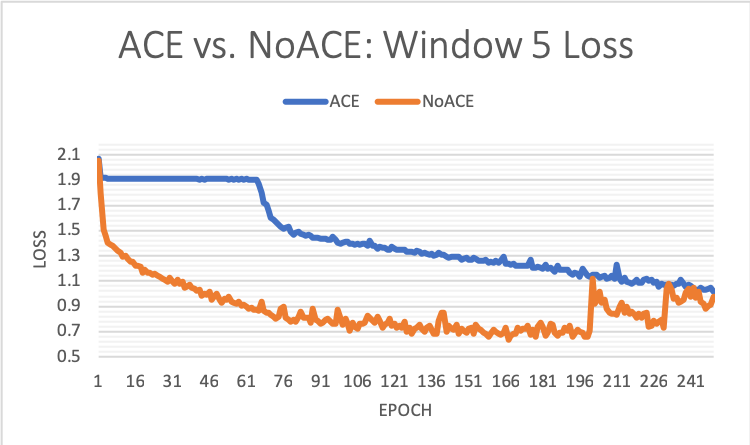
\includegraphics[width=\linewidth]{acevnoace-window5-loss.png}
		\caption{Window Size 5 Training Loss}
	\end{subfigure}
	\hfill
	\begin{subfigure}{0.45\linewidth}
		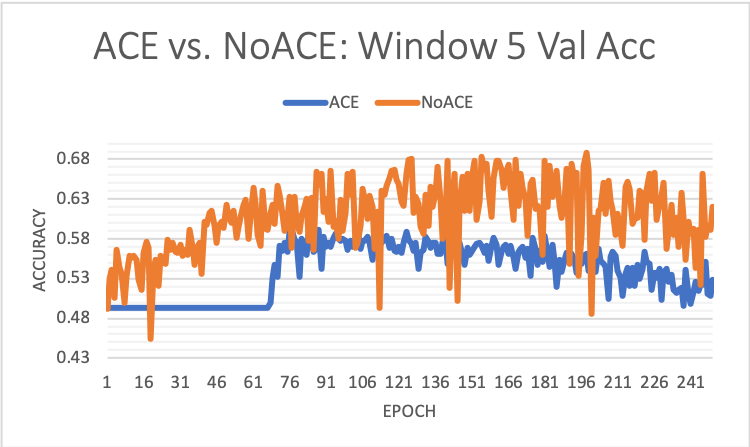
\includegraphics[width=\linewidth]{acevnoace-window5-valacc.png}
		\caption{Window Size 5 Validation Accuracy}		
	\end{subfigure}


	\begin{subfigure}{0.45\linewidth}
		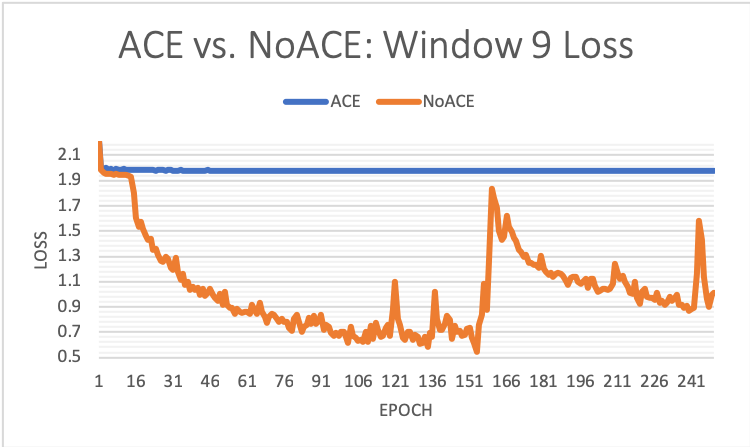
\includegraphics[width=\linewidth]{acevnoace-window9-loss.png}
		\caption{Window Size 9 Training Loss}
	\end{subfigure}
	\hfill
	\begin{subfigure}{0.45\linewidth}
		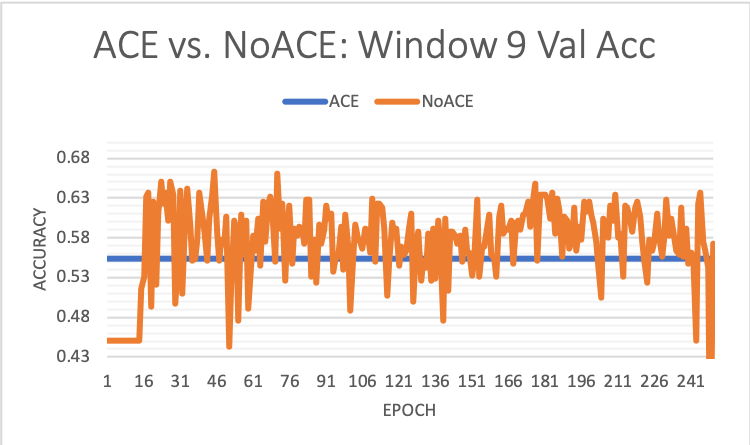
\includegraphics[width=\linewidth]{acevnoace-window9-valacc.png}
		\caption{Window Size 9 Validation Accuracy}		
	\end{subfigure}
	

\end{figure*}


After reviewing previous experiment results and observing that the loss was minimized with a window size of 9 for both ACE Disabled and ACE Enabled, but also seeing that the networks were not diverging, I ran an experiment with the same parameters as the previous, except I trained the networks for 250 epochs, and I lowered the stride from $\lfloor\frac{w}{2}\rfloor = 4$ to 3, thus increasing training time, but also increasing the number of training samples. 
%
I ran this experiment with both ACE Enabled and ACE Disabled to see how the ACE approach altered validation accuracy. 

Because loss was minimized with window size 9, and validation accuracy was maximized with window size 5, I decided to run this experiment twice: once with window size 5 and once with window size 9.
%
The results of this experiment are shown in Figure \ref{figure:acevnoace}.

When looking at the results of the second set of experiments, I see two common trends.
%
The first is that the NoACE experiments are overall better performing than the ACE experiments in general.
%
The loss of NoACE is lower than the loss of ACE and the validation accuracy is higher for NoACE than for ACE for the majority of epochs of training.
%
Recall that I chose to train for 250 epochs instead of 100 to allow the ACE experiments to converge, but I again see that ACE does not converge.
%
There is no asymptotic behavior of the loss function like I wanted to see.
%
In fact, the loss never changes past the 5th epoch for window size of 9, indicating that the network is not learning the provided data.
%
While overall I notice that NoACE performs better, the second trend I observe is that the ACE experiments are more consistent than the NoACE.
%
The NoACE experiments behave with a lot of oscillation, both in loss and validation accuracy, which means that while overall they perform better, I cannot put trust or credibility into seeing results after a given epoch because the numbers following the next epoch may not follow the trend.
%
The ACE Enabled experiments on the other hand generally had loss decrease (or remain the same) epoch over epoch and validation accuracy increase epoch over epoch. 
%
The results of this experiment show that ACE does not benefit CNN performance in HSI classification using my current method, but rather hinders it.
%
Perhaps using ACE Global on each patch with the mean signals would be perform better than using a window size of 3 in ACE Local.

\subsection{Ideal Network Size}

\begin{table*}[t]
	
	\centering
	
	\caption{CNN Performance with Varied Number of Convolutional Layers}
	\label{table:cnn}
	\begin{tabular}{l | c | c }
		\textbf{No. Layers} & \textbf{ACE} & \textbf{NoACE} \\			
		\hline	
		1 & 0.5234 & 0.7357 \\
		5 & 0.4163 & 0.7010 \\
		15 & 0.5439 & 0.6306 \\
		25 & 0.5327 & 0.4337 \\
		50 & 0.5327 & 0.5184 \\
		
	\end{tabular}	
	
\end{table*}


\begin{figure*}[t]
	
	\centering
	\caption{Classification accuracy with various number of convolutional layers}
	\label{figure:num-layers}
	
	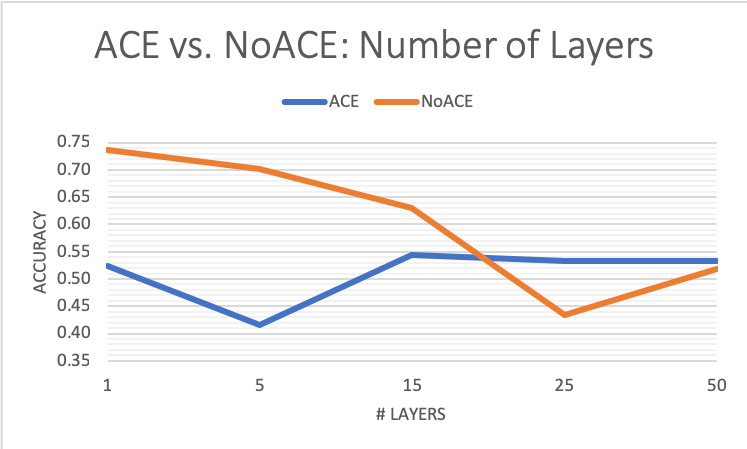
\includegraphics[width=0.5\linewidth]{num-layers.png}
	
	
	
\end{figure*}

Following experiments to determine the utility of ACE Local on CNN classification performance and identify the optimal CNN input size, I decided to run an experiment to investigate the relationship between number of convolutional layers and CNN performance, both with and without ACE.
%
For this experiment, I choose to use an input window size of 5 with a stride of two based on previous experiments result.
%
I then hold everything else constant and consistent with previous experiments, and only vary the number of convolutional layers.
%
I vary this parameter from 1 up to 50, and train each network for 250 epochs.
%
The results of this experiment are shown in Table \ref{table:cnn} and Figure \ref{figure:num-layers}.

In reviewing the results of the ideal network size experiment, I see that the ideal network size is different with and without ACE.
%
Without ACE, the ideal network size is only 1 convolutional layer.
%
This result is surprising because HSI have more bands than RGB, but is not surprising for this dataset, as all classes are agricultural. 
%
I am not discriminating between airplanes and churches and roads, but instead on different agricultural features, so perhaps the features needed to classify these features can be extracted in 1 convolutional layer for this dataset.
%
With ACE enabled, we see that the ideal network size is 15. 
%
This indicates to me a kind of Goldilocks situation, where 1 is too few, 50 is too many, and 15 is in that "just right" range. 
%
These results also show that as the number of convolutional layers increase without ACE, the worse the classification results are, with the exception of 50 layers, which sees an increase over 25.
%
I also see that for a number of layers greater than or equal 25, ACE does outperform the NoACE mode, which is odd because the ACE mode has only 16 bands whereas NoACE has 220, so I expected more bands to need more convolution to extract the features more efficiently, but that is not the case.
%
The results show that the ACE data is more complex feature wise than the NoACE data, so the spectral information is harder to extract than the spatial information in the NoACE version, which is intuitive, but is also counterintuitive given the discrepancy in number of bands.

%5) CONCLUSIONS. summarize it folks!
\section{Conclusion}\label{sec:conclusion}
In conclusion, the addition of ACE preprocessing to a Convolutional Neural Network for Hyperspectral Image classification did not benefit classification performance. 
%
In addition, the choice of window size is a key parameter for HSI classification, and too large of a window size will result in terrible classification performance due to the overwhelming amount of context. 
%
While window size is an important choice for HSI classification, an even more crucial decision is the number of convolutional layers.
%
For the benchmark Indian Pines hyperspectral dataset, the choice of too many convolutional layers reduced validation accuracy from 0.74 down to 0.43, a reduction of more than 30\% in classification accuracy.
%
The result of several experiments showed that following ACE, the features of spectral data were more complex and therefore when more epochs and more convolutional layers were used, an increase in performance was seen.
%
Continued research for this project would include the usage of different ACE window sizes as well as an investigation into how ACE Global performed rather than ACE local.
%
Further, an investigation into if the conclusions drawn here would hold for other hyperspectral datasets would be an important next step to ensure work here is not too specified for Indian Pines.
%
Overall, the use of ACE caused a decrease in classification performance when compared with a standard CNN, but additional parameter and training schemes could potentially flip the script if the correct configuration was found.


%%%%%%%%%%%%%%%%
%		 REFERENCES
%%%%%%%%%%%%%%%%%

\bibliography{refs} 
\bibliographystyle{ieeetr}


\end{document}
